\section{Implementierung}
Dies Kapitel dient dazu nachzuvollziehen, wie sich das Programm im Web verhalten würde. Um zu gewährleisten, dass das Programm bei misverhalten keinen Schaden an dem gerade getesteten Forum anrichtet, wird ein eigenes Forum aufgebaut, ein vollständiger Arbeitszyklus, lokal an diesem Forum getestet.

\subsection{Implementierungsumgebung}
Das Forum Zugriff auf eine Datenbankquelle haben. Diese besteht für die Dauer der Tests, aus einem Teil der Noise to Opportunity Datenbank mit 50.000 Einträgen. Diese Einträge umfassen einen Posttitel , einen Postinhalt und eine eindeutige Weburl, die als ID benutzt wird. Die Posts sind in einer NoSQL-Datenbank, Elasticsearch, gespeichert. Diese bietet den Vorteil, das mit nur einer Anfrage an die Datenbank in Posttitel und Postinhalt, leicht nach einem bestimmten Suchwort gesucht werden kann, und die ersten 20 gefundenen Posts zurückgeliefert werden können.\\
Das Forum wird lokal erstellt, um eine Vielzahl an Anfragen an ein im Internet verfügbares Forum zu vermeiden. Eine ordentliche Evaluierung könnte diesem Forum durch zu viel Netzwerkverkehr eventuell schaden.\\
Geschrieben werden alle Programme, die die Thesen umsetzen, mit Hilfe von JavaScript. Das Forum wird auf einem node\.js-Server laufen. 
\subsubsection{Aufbau des Forums}
Das Forum sollte einem originalen Internetforum möglichst nahe kommen, jedoch gleichzeitig eine Umgestaltung der einzelnen Seiten für Anmelden, Registrieren und Suchen nicht allzu aufwändig machen. Dieses erlaubt ein schnelles debuggen, wenn sich das Programm nicht wie erwartet verhält. Deshalb wird sich bei dem Erstellen des Forums auf die wichtigsten Elemente konzentriert. Diese umfassen eine Login-, eine Registrierungs- und eine Suchseite.
\subsubsection{Registrierung im Forum}
Die häufigste Registrierungsform die man in diversen Internetforen findet bestehen aus 2 Feldern für das Passwort, 2 Feldern für die Email, einem Feld für den Nutzernamen und eine Checkbox, dass die Foren-AGB angenommen werden. Dieses wird simpel durch das folgende Codebeispiel nachgebaut.

\begin{figure}[h!]
\begin{lstlisting}[language=HTML5]
<form action="/reg" method="post">
Nutzername: <input type="text" name="fname"></br>
Email: <input type="text" name="email"></br>
Validate Email: 
<input type="text" name="re_email"></br>
Password: <input type="password" name="pwd"></br>
Validate Password: 
<input type="password" name="re_pwd"></br>
Accept AGB:<input type="checkbox" name="AGB"></br>
<input type="hidden" name="val1" value="val1">
<input type="hidden" name="val2" value="val2">
<input type="submit" value="Submit">
</form>
\end{lstlisting}
\caption{HTML-Code für die Erstellung einer Registrierungsseite, mit Nutzernamen, Email und Passwordfeldern, sowie Checkbox}
\end{figure}
\newpage

Aus Figure 1 ist es leicht zu Evaluieren, ob der Registrierungsprozess erfolgreich sein würde. Zu erwaren wäre ein POST-Request an die Toplevel Domain + Formaction mit den Postparametern fname, email, re\_email, pwd, re\_pwd, AGB, sowie den hidden Key-Value-Pairs, val1=hiddenvalue1 und val2=hiddenvalue2.\\
In die Postparameter sollten in die entsprechenden Felder, fname, email und pwd jeweils der Name, die Email und das Passwort eingetragen, sowie in den re\_email, re\_pwd jeweils die Email bestätigt und das Passwort bestätigt sein, indem sie nochmals eingetippt sind.\\
Ist der HTTP-Server gestartet und wird die Registrierungsseite analysiert und der folgende Request an den Server gesendet :

\begin{figure}[ht]
\begin{lstlisting}[language=HTML5]
/reg
{ val2: 'hiddenvalue2',
val1: 'hiddenvalue1',
AGB: 'on',
re_pwd: 'AjZt198#ev',
pwd: 'AjZt198#ev',
re_email: 'jpm96353@adiaq.com',
email: 'jpm96353@adiaq.com',
fname: 'Dominik' }
verification email to : jpm96353@adiaq.com
\end{lstlisting}
\caption{Inhalt des Post-Requests, den der Client an das Forum bei einem Registrierungsaufruf sendet}
\end{figure}

Zu verzeichnen ist, dass sich der Client eine eigene Email angelegt hat, diese stammt von der Internetseite 10minutemail\footnote{https://10minutemail.net/ checked: 10.06.2015}.
Diese Internetseite, stellt für 10 Minuten eine kostenlose Emailadresse zur Verfügung, mit der Emails empfangen und gesendet werden können. Die Registrierungsaufforderung wurde an die richtige Url des Servers gesendet, welches aus dem /reg ersichtlich wird. Weiterhin sind alle erforderlichen Parameter des Post-Requestes entsprechend ausgefüllt, und auch die Wiederholungsfelder von Email und Passwort sind korrekt ausgefüllt. Die Checkbox für die AGB ist angekreuzt worden und auch alle versteckten Input-Felder der Form mit übertragen. Insgesamt ist dieses eine gültige Registrierungsanfrage, welche der Server mit einer Validierungsemail an die angegebene Emailadresse quittiert.

Der Client überprüft alle 5 Sekunden ob die Email eingegangen ist. Sollte dieses der Fall sein wird der Link zu der Email aufgerufen, die Email analysiert und jeder darin befindliche Link aufgerufen. Sollte innerhalb von 10 Minuten keine neue Email eingegangen sein, wird der Registrierungsversuch als gescheitert angesehen und dem Nutzer mitgeteilt, denn die Emailadresse ist nur 10 Minuten valide.

\begin{figure}[ht]
\begin{lstlisting}[language=HTML5]
registered
No new emails
No new emails
No new emails
location='readmail.html?mid=KfKcm0'
https://10minutemail.net/readmail.html?mid=KfKcm0
clicked: http://localhost:12345/validateUser?user=jpm96353@adiaq.com
\end{lstlisting}
\caption{Client wartet auf Registrierungsemail und ruft alle Links in der Email auf.}
\end{figure}

Der Validierungsversuch wird nun an das Forum gesendet, welches den Nutzer als aktiven Nutzer validiert.

\begin{figure}[ht]
\begin{lstlisting}[language=HTML5]
/validateUser?user=jpm96353@adiaq.com
validate:
jpm96353@adiaq.com
\end{lstlisting}
\caption{Forum validiert den Nutzeraccount, da Validierungslink bestätigt wurde.}
\end{figure}

Sollte der Registrierungsprozess nicht funktionieren, kann die Registrierungsform nachgebaut werden, gegeben falls Änderungen an den Feldbewertungsmetriken gemacht werden und dann erneut ausprobieren, ohne Webforen zu belasten. Es gibt auch die Möglichkeit für das Programm den Registrierungsschritt zu überspringen, wenn der Nutzer schon einen Nutzeraccount per Hand angelegt hat, kann er das dem Programm über Eingabeparameter mitteilen. Anstatt sich neu zu registrieren, nutzt er nun den vorhandenen Nutzeraccount.

\subsubsection{Forenlogin}
Der Forenlogin sollte bei nicht angegebenen Logindaten mit den zuvor generierten Daten ausgeführt werden, werden Daten angegeben sollten diese auch benutzt werden. Der Loginrequest sollte 3 Parameter enthalten, einmal den Nutzernamen und einmal das Passwort. Die Checkbox gibt an ob man auf der Website eingeloggt bleiben möchte, um bei einem späteren Besuch nicht nochmal die Nutzerdaten eingeben zu müssen. Das sind die gängigsten Loginformulare, die im Internet herrschen.

\begin{figure}[ht]
\begin{lstlisting}[language=HTML5]
<form action="/log" method="post">
Nutzername: 
<input type="text" name="fname"></br>
Password: 
<input type="password" name="pwd"></br>
Eingeloggt bleiben: 
<input type="checkbox" name="remember">
<input type="submit" value="Submit">
</form>
\end{lstlisting}
\caption{HTML-Code der die Loginseite des Forums erstellt}
\end{figure}
\newpage

\begin{figure}[h!]
\begin{lstlisting}[language=HTML5]
loginattempt: 
{fname:'Dominik',
remember: 'on',
pwd:'AjZt198#ev'}
\end{lstlisting}
\caption{Eingehende Loginanfrage des Clients im Forum}
\end{figure}

In Figure 6 ist zu sehen, dass alle erforderlichen Daten korrekt ausgefüllt wurden.

\begin{figure}[h!]
\begin{lstlisting}[language=HTML5]
loginattempt:
{email: 'jpm96353@adiaq.com',
fname: 'Dominik',
remember: 'on',
pwd: 'AjZt198#ev'}
\end{lstlisting}
\caption{Eingehende Loginanfrage des Clients im Forum, mit Nutzername und Email}
\end{figure}
Figure 7 zeigt, dass wenn die Loginform Usernamen und Email abfragen sollte, wird ein valider Loginrequest abgesendet wird.

\begin{figure}[h!]
\begin{lstlisting}[language=HTML5]
loginattempt:
{email: 'jpm96353@adiaq.com',
fname: 'Dominik',
remember: 'on',
pwd: 'AjZt198#ev',
hiddenvalue: 'v1'}
\end{lstlisting}
\caption{Eingehende Loginanfrage des Clients im Forum, mit versteckten Attributen}
\end{figure}

Auch etwaige versteckte Input-Felder werden korrekt gefunden und die Key-Value Paare in dem POST-Request mit übergeben (Figure 8).
\newpage

Alle nachgebauten Loginseiten diverser im Internet gefundenen Seiten wurden im händischen Test erfolgreich ausgefüllt und die zu erwartende Loginanfrage an den Server gesendet.\\
Es ist programmatisch möglich sich in Foren automatisch zu registrieren und anzumelden. Um die erste Theorie vollständig zu evaluieren müssen nach dem Loginvorgang nun noch relevante Posts zu den jeweiligen Firmenprodukten aus dem Forum extrahiert werden.\\
Hierzu werden in Internetforen die Nutzer, die sich gerade angemeldet haben, auf die Hauptseite des Forums verwiesen. Damit der Browser das realisiert, wird in der Antwort des Servers nach dem erfolgreichen anmelden, ein Statuscode 302 gesendet. Dieser zeigt an, das der Browser eine andere Url ohne das Zutun des Nutzers laden soll. Die Url steht im Location-Header der Antwort. Dieses muss programmatisch realisiert werden, da sonst, ohne den Redirect, bei einer Analyse des HTML Quellcodes keine Suchform gefunden werden könnte, da immer die vorherige, also die Login-Seite analysiert werden würde.\\
Der Server antwortet auf eine erfolgreiche Loginanfrage mit einem Redirect.

\begin{figure}[ht]
\begin{lstlisting}[language=HTML5]
successfull login from: jpm96353@adiaq.com
send 302 to redirect to /main
/main
\end{lstlisting}
\caption{Erfolgreicher Login im Forum und Redirect des Clients zur Hauptseite}
\end{figure}

Der Client überprüft bei jeder Anfrage an den Server ob der Statuscode sich von 200 (OK) unterscheidet. Sollte es wie in diesem Fall ein 302 (Redirect) sein, wird automatisch die neue Url mit einem Get-Request nachgeladen, damit das neue HTML analysiert werden kann im nächsten Schritt. In diesem Fall wird die Main- Page des Forums als nächstes geladen.

\newpage

\subsubsection{Suchen im Forum}
\begin{figure}[ht]
\begin{lstlisting}[language=HTML5]
http://localhost:12345/log
{ email: 'jpm96353@adiaq.com',
fname: 'Dominik',
pwd: 'AjZt198#ev',
hiddenvalue: 'v1' }
redirected
redirecturl: /main
\end{lstlisting}
\caption{Client folgt dem Redirect auf die Hauptseite des Forums}
\end{figure}

Der Client erkennt automatisch das er auf eine andere Seite verwiesen wurde und lädt diese. Dieses ist daran zu erkennen, dass das HTML was im nächsten Schritt analysiert wird nicht mehr das Login-HTML ist.

\begin{figure}[h!]
\begin{lstlisting}[language=HTML5]
<form accept-charset="UTF-8" action="/search" class="js-site-search-form" data-global-search-url="/search" data-repo-search-url="" method="get">
<div style="margin:0;padding:0;display:inline">
<input name="utf8" type="hidden" value="true"></div>
<label class="js-chromeless-input-container form-control">
<input type="text" class="js-site-search-focus chromeless-input" data-hotkey="s" name="q" placeholder="Search OwnForum" data-global-scope-placeholder="Search OwnForum" data-repo-scope-placeholder="Search" tabindex="1" autocapitalize="off">
</label>
</form>
\end{lstlisting}
\caption{Zu analysierendes HTML nach dem Redirect, enthält die Suchform}
\end{figure}

Dieses HTML wird nach einer Suchform durchsucht. Diese befindet sich meist ein einer Get-Form. Da der Request ein get Request ist wird das Suchwort in der Url codiert. Der Name des Key-Value-Paares, welches für die Übermittlung zuständig ist, wird aus den Input-Feldern in der Form generiert. Dieses Attribut hat meist in den Namen `q` oder `search`. Der Client findet diese Suchform und sendet die Suchanfrage an den Server.


\begin{figure}[ht]
\begin{lstlisting}[language=HTML5]
{ action: '/search', name: 'q' }
\end{lstlisting}
\caption{Vom Client analysierte Suchform, gefundener Name des Suchparameters und die Suchurl}
\end{figure}

In dem Forum geht eine valide Suchanfrage ein.


\begin{figure}[ht]
\begin{lstlisting}[language=HTML5]
/search?q=CRM
/search?q=LVM
/search?q=HCM
/search?q=ECOM
\end{lstlisting}
\caption{Eingehende Suchanfragen im Forum }
\end{figure}

Diese Suchwörter werden in dem Forum gesucht. Sollte das Suchwort in dem Titel oder dem Postcontent vorkommen, wird der Link zu diesem Post zurückgegeben. Dieser Link ist in dem Testforum eine eindeutige ID. Es ist anzunehmen das die Links eine eindeutige ID für jeden Post darstellen, da sie auf genau eine feste Internetadresse verweisen. So wie in einem Internetforum werden pro Suchwort die ersten 20 Treffer zu diesem Suchwort auf einer HTML zusammengefasst und an den Client ausgeliefert. Zu erwarten ist, dass der Client alle Links speichert und vermerkt wie oft der Link bei unterschiedlichen Suchworten von dem Forum zurückgegeben wurde. Dazu wird das HTML nach allen vorkommenden Links durchsucht. Des weiteren sollten Links die in mehr als der Hälfte der Suchanfragen wiedergegeben werden, da es sich hierbei meist um statische Links handelt wie neuste Posts oder Links in den Navigationsleisten, entfernt werden.
\newpage

\begin{figure}[h!]
\begin{lstlisting}[language=JavaScript]
dispatcher.onGet("/search", function(req, res) {
res.writeHead(200, {'Content-Type': 'text/html'})
var results = searchDataBaseForWord(req.params.q)
.then(function(results){
if(results.length > 0){
var temp = ''
for (var i = results.length - 1; i >= 0; i--) {
temp += '<a href="/'+ results[i] +'">Link</a>'
temp += '</br>'
}
temp +='<a href="/shouldberemovedLink">REMOVELINK</a>'
temp += '</br>'
res.write(temp)
}else{
var temp = ''
temp +='<a href="/shouldberemovedLink">REMOVELINK</a>'
temp += '</br>'
temp += "<h1> No valid Data found </h1>"
res.write(temp)
}
res.end() 
}) 
})
\end{lstlisting}
\caption{Erstellung der Ergebnisseite auf eine Suchanfrage im Forum}
\end{figure}

In Figure 14 wird für jede Suchanfrage das HTML erstellt, das die Links zu den jeweiligen passenden Dokumenten enthält. Diese Links stammen aus der Datenbankabfrage mit dem entsprechenden Suchwort.
Ein statischer Link wird platziert. Dieser soll die statischen Links auf Internetseiten simulieren, welcher dann von dem Client entfernt werden sollte, da er in mehr als der Hälfte der Anfragen vorhanden ist und somit wahrscheinlich kein Link zu einem Post darstellt.

\begin{figure}[h!]
\begin{lstlisting}[language=HTML5]
/search?q=besiege
/search?q=briar
/search?q=individuals
/search?q=evacuate
/search?q=steals
/search?q=detrimental
/search?q=untimely
/search?q=bestir
/search?q=graphical
/search?q=revelation
\end{lstlisting}
\caption{10 Suchanfragen des Clients an das Forum, mit zufälligen Wörtern}
\end{figure}

\begin{figure}[h!]
\begin{lstlisting}[language=HTML5]
{"href=\"/g-1814892-S-5993338243263848452\"":1,
"href=\"/g-1850237-S-6005730948694503428\"":1,
"href=\"/g-115178-S-5999229826848821253\"":1,
"href=\"/g-66325-S-6001320511865446402\"":1,
"href=\"/g-66325-S-6003599070168440836\"":1,
"href=\"/g-54723-S-5999922118567956482\"":1}
\end{lstlisting}
\caption{Gesammelte Dokumente des Clients auf die 10 Suchanfragen}
\end{figure}

Bei 10 Suchanfragen an die Datenbank (Figure 15), mit zufälligen englischen Wörtern wurden 6 Dokumente in der Testdatenbank gefunden (Figure 16). Keines wurde doppelt getroffen und der statische Link wurde entfernt. Die verbleibenden Links können nun mit einem GET-Request an den entsprechenden Link heruntergeladen und indexiert werden.
\newpage

\begin{figure}[h!]
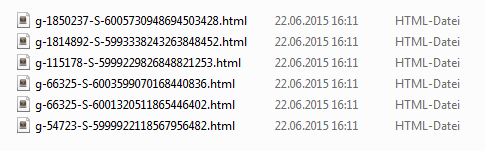
\includegraphics{./images/postdownload.png}
\caption{Heruntergeladne HTML-Seiten der Posts der Suchanfragen}
\end{figure}


Es wurden erfolgreich die 6 Dokumente des Forums heruntergeladen, die das Forum auf die 10 Suchanfragen ausgeliefert hat.
Damit ist gezeigt, das es möglich ist sich automatisch in Foren zu registrieren , einzuloggen und nach bestimmten (firmenspezifischen) Schlagworten für Produkte zu suchen.

\subsubsection{Bestimmung der Forenrelevanz}

Es geht darum zu evaluieren, ob eine Vorhersage darüber zu treffen, wie groß eine Forendatenbank ist und wie relevant dieses Forum für ein jeweiliges Unternehmen ist, erfüllbar ist.

Es wird zunächst die Datenbankgröße bestimmt wie in Kapitel [] beschrieben. Die Testdatenbank wurde in 3 Segemente geteilt. Segement 1 enthält nur Posts aus Forum 1, Segement 2 nur aus Forum 2 und Segement 3 nur Posts aus Forum 3. 
Segement 1 und 2 beinhalten englische Posts, wohingegen Segement 3 meist deutsche Posts enthält. Die Postanzahl aller 3 Segemente ist bekannt. Um eine realistische Einschätzung zu erhalten, wie zuverlässig die Vorhersage der Gesamtdatenbankgröße ist, wurde der Test für jedes Segement 3 mal wiederholt. Ein Testdurchlauf besteht aus 3 mal 500 zufälligen Wörtern, die an die Datenbank in der passenden Sprache gesendet werden. Die ermittelten Datenbankgrößen nach 500 Wörtern werden addiert und durch die Gesamtanzahl der Testläufe dividiert und danach mit der bekannten Gesamtanzahl der Posts in dem Datenbanksegment verglichen.

\begin{table}[h!]
\begin{tabular}{ | p{3cm} | p{3cm} | p{3cm}| p{3cm} |} \hline
Durchlauf & Anzahl Dok in S1 & Anzahl Dok in S2 & Anzahl Dok in S3 \\ \hline
1 & 12572 & 18374 & 8079 \\ \hline
2 & 10400 & 21155 & 7896 \\ \hline
3 & 15017 & 20952 & 8343 \\ \hline
Arith. Mittel & 12663 & 20160 & 8016 \\ \hline
org. Größe & 12133 & 21221 & 8184 \\ \hline
Fehler & +4\% & -5\% & -1\% \\ \hline
\end{tabular}
\caption{Ermittelung der Datenbankgrößen mit zufälligen Wörtern}
\end{table}

\newpage

Der Fehler beträgt maximal 5\% , dieses bestätigten die zwei weiteren Testdurchläufe. Damit ist eine Voraussage einer Forendatenbank bis auf 10\% Differenz genau möglich sein.

Im nächsten Schritt sollen die einzelnen Produkte in dem Forum gesucht werden. Dazu werden, wie in Kapitel[] beschrieben, beschreibende Wörter für jedes einzelne Produkt generiert. Diese Keywords werden gesucht und die Datenbankgröße aufgrund des Verhältnisses zwischen überlappenden und einzigartigen Dokumenten, wie in Kapitel[] beschreiben, berechnet. Die Datenbank die zu Testzwecken verwendet wurde enthält 21220 Posts.

\begin{table}[h!]
\begin{tabular}{ | p{3cm} | l |}
\hline
Produkt & Anzahl der Dokumente in DB \\ \hline
CRM & 2386 \\ \hline
HCM & 3138 \\ \hline
ECOM & 3641 \\ \hline
LVM & 1769 \\ \hline
Gesamt & 10934 \\ \hline
\end{tabular}
\caption{Anzahl der Dokumente je Kategorie in der Testdatenbank. Der Rest der Posts konnte keinem Produkt eindeutig zugeordnet werden.}
\end{table}

\newpage

\begin{table}[h!]
\begin{tabular}{ | p{3cm} | l | l |}
\hline
Produkt & Berechnete Anzahl der Dokumente in DB & Fehler\\ \hline
CRM & 3800 & +59 \%\\ \hline
HCM & 9668 & +338 \% \\ \hline
ECOM & 10604 & +265 \%\\ \hline
LVM & 39541 & +2235 \%\\ \hline
\end{tabular}
\caption{Errechnete Datenbankgröße nach Produkt mit Suchworten nach tf-idf Maß}
\end{table}

Zu verzeichnen ist das die Größe der einzelnen Produktkategorien maßlos überschätzt wurde. Deshalb wird zur Ergebnisverbesserung ein zusätzlicher Schritt eingefügt. Es werden wie bisher die Keywords zu den jeweiligen Produkten im Forum gesucht, jedoch bevor der Post zur Berechnung des Gesamtkorpus beiträgt, durch einen Klassifizierungsservice \cite{n2o} analysiert. Dieser bestimmt aus einem gegebenen Text, auf Grundlage der selben Broschüren, die zur Berechnung der tf-idf- Keywords verwendet werden, welchem Produkt der Post am ehesten entspricht.

\begin{figure}[h!]
\begin{lstlisting}[language=HTML5]
http://192.168.42.54:9001/predictions?text=Hi, I want to by an CRM product
\end{lstlisting}
\caption{Senden eines Testtextes an den Analyseservice}
\end{figure}

\newpage

\begin{figure}[h!]
\begin{lstlisting}[language=HTML5]
{
"product": [
{
"product": "CRM",
"prob": 0.9999979024787202
},
{
"product": "ECOM",
"prob": 0.0000020975212798552666
},
{
"product": "LVM",
"prob": 3.0982005787342066e-25
},
{
"product": "None",
"prob": 2.2462124385020632e-66
},
{
"product": "HCM",
"prob": 1.5018464896178129e-218
}
]
}
\end{lstlisting}
\caption{Antwort des Analyseservices mit entsprechender Klassifizierung des Textes}
\end{figure}

Der Posttext (Figure 18) würde als CRM Post richtig eingestuft werden. Wenn gerade die CRM Forendatenbankgröße berechnet werden sollte, wird dieser Post mit in die Berechnung einfließen. Alle Post die als nicht CRM Posts eingestuft werden, werden in dieser spezifischen Ermittlung nicht betrachtet.\\
Mit maximal 100 generierten Keywords gewichtet nach der höchsten tf-Idf werden folgende Resultate erreicht.

\begin{table}
\begin{tabular}{ | p{3cm} | l | l |}
\hline
Produkt & Berechnete Anzahl der Dokumente in DB & Fehler \\ \hline
CRM & 2270 & -5\% \\ \hline
HCM & 2730 & -14 \% \\ \hline
ECOM & 4388 & +17\% \\ \hline
LVM & 1670 & -5\% \\ \hline
\end{tabular}
\caption{Errechnete Datenbankgröße je Produkt mit sortierten tf-idf Wörtern und Analyseservice}
\end{table}

Die anderen 2 Testsegmente der Datenbank konnten mit ähnlich genauen Fehlern überprüft werden.
Ein Fehler von maximal 20\% mit nur maximal 100 Suchanfragen ist eine zufriedenstellende Größe. Aus der Datenbankgröße und den spezifischen Produktdatenbankgrößen lässt sich bestimmen ob das Forum zum Verkauf eines Produktes geeignet ist oder nicht.
